\documentclass[11pt]{article}
%\hypersetup{colorlinks}% uncomment this line if you prefer colored hyperlinks (e.g., for onscreen viewing)

%\geometry{showframe}% for debugging purposes -- displays the margins

\newcommand{\E}{\mbox{E}}
\newcommand{\MSE}{\mbox{MSE}}
\newcommand{\var}{\mbox{var}}

\usepackage{amsmath,amssymb,amsfonts,amsthm} % amsmath package, useful for mathematical formulas
%\usepackage[garamond]{mathdesign}
\usepackage{url}

\newtheorem{theorem}{Theorem}
\newtheorem{lemma}[theorem]{Lemma}

% Set up the images/graphics package
\usepackage{graphicx}
\setkeys{Gin}{width=\linewidth,totalheight=\textheight,keepaspectratio}
\graphicspath{{graphics/}}

\title{Exercises 6 $\cdot$ SDS 383D \\ Exercises 6: Linear smoothing and Gaussian processes}
%\author[ ]{ }
\date{}  % if the \date{} command is left out, the current date will be used

% The following package makes prettier tables.  We're all about the bling!
\usepackage{booktabs}

% The units package provides nice, non-stacked fractions and better spacing
% for units.
\usepackage{units}

% The fancyvrb package lets us customize the formatting of verbatim
% environments.  We use a slightly smaller font.
\usepackage{fancyvrb}
\fvset{fontsize=\normalsize}

% Small sections of multiple columns
\usepackage{multicol}

% Provides paragraphs of dummy text
\usepackage{lipsum}

% These commands are used to pretty-print LaTeX commands
\newcommand{\doccmd}[1]{\texttt{\textbackslash#1}}% command name -- adds backslash automatically
\newcommand{\docopt}[1]{\ensuremath{\langle}\textrm{\textit{#1}}\ensuremath{\rangle}}% optional command argument
\newcommand{\docarg}[1]{\textrm{\textit{#1}}}% (required) command argument
\newenvironment{docspec}{\begin{quote}\noindent}{\end{quote}}% command specification environment
\newcommand{\docenv}[1]{\textsf{#1}}% environment name
\newcommand{\docpkg}[1]{\texttt{#1}}% package name
\newcommand{\doccls}[1]{\texttt{#1}}% document class name
\newcommand{\docclsopt}[1]{\texttt{#1}}% document class option name

\newcommand{\N}{\mbox{N}}
\newcommand{\thetahat}{\hat{\theta}}
\newcommand{\sigmahat}{\hat{\sigma}}
\newcommand{\betahat}{\hat{\beta}}

%% ys
\usepackage[shortlabels]{enumitem}
\usepackage{geometry}
\usepackage{bm}
\usepackage{amssymb}
\usepackage{algorithm}
\usepackage{algpseudocode}
\usepackage{xcolor}
\usepackage{listings}
\geometry{a4paper,scale=0.75}
\newcommand{\jie}{$\star$ }
\renewcommand{\bx}{\bm{x}}
\newcommand{\iid}{\overset{\text{iid}}{\sim}}
\newcommand{\half}{\frac{1}{2}}
\newcommand{\ynote}[1]{\color{red} #1 \color{black}}

\usepackage{graphicx}
\usepackage{fancyvrb}
\usepackage{listings}
\usepackage{bm}
\usepackage{xcolor}
\usepackage{caption}
\usepackage{subcaption}
\usepackage{graphicx}

\xdefinecolor{gray}{rgb}{0.4,0.4,0.4}
\xdefinecolor{blue}{RGB}{58,95,205}% R's royalblue3; #3A5FCD

\lstset{% setup listings
	language=R,% set programming language
	basicstyle=\ttfamily\small,% basic font style
	keywordstyle=\color{blue},% keyword style
        commentstyle=\color{gray},% comment style
	numbers=left,% display line numbers on the left side
	numberstyle=\scriptsize,% use small line numbers
	numbersep=10pt,% space between line numbers and code
	tabsize=3,% sizes of tabs
	showstringspaces=false,% do not replace spaces in strings by a certain character
	captionpos=b,% positioning of the caption below
        breaklines=true,% automatic line breaking
        escapeinside={(*}{*)},% escaping to LaTeX
        fancyvrb=true,% verbatim code is typset by listings
        extendedchars=false,% prohibit extended chars (chars of codes 128--255)
        %literate={"}{{\texttt{"}}}1{<-}{{$\bm\leftarrow$}}1{<<-}{{$\bm\twoheadleftarrow$}}1
        %{~}{{$\bm\sim$}}1{<=}{{$\bm\le$}}1{>=}{{$\bm\ge$}}1{!=}{{$\bm\neq$}}1{^}{{$^{\bm\wedge}$}}1,% item to replace, text, length of chars
        alsoletter={.<-},% becomes a letter
        alsoother={\$},% becomes other
        otherkeywords={!=, ~, \$, \&, \%/\%, \%*\%, \%\%, <-, <<-, /},% other keywords
        deletekeywords={c}% remove keywords
}
%% ys

\begin{document}

\maketitle% this prints the handout title, author, and date


\section{Basic concepts}

\subsection{Bias--variance decomposition}

Let $\hat{f}(x)$ be a noisy estimate of some function $f(x)$, evaluated at some point $x$.  Define the mean-squared error of the estimate as
$$
\MSE(\hat{f}, f) = \E\{ [ f(x) - \hat{f}(x)]^2 \} \, .
$$
A simple derivation shows that $\MSE(f, \hat{f}) = B^2 + v$, where
$$
B = \E \{ \hat{f}(x) \} - f(x) \quad \mbox{and} \quad V = \var\{ \hat{f}(x) \} \, .
$$
This is the bias--variance decomposition of mean-squared error.

\subsection{A simple example  (optional problem)}

Some people refer to the above decomposition as the \textit{bias--variance tradeoff.}  Why a tradeoff?  Here's a simple example to convey the intuition.

Suppose we observe $x_1, \ldots, x_n$ from some distribution $F$, and want to estimate $f(0)$, the value of the probability density function at 0.  Let $h$ be a small positive number, called the \textit{bandwidth}, and define the quantity
$$
\pi_h = P\left( -\frac{h}{2} < X < \frac{h}{2} \right) = \int_{-h/2}^{h/2} f(x) dx \, .
$$
Clearly $\pi_h \approx h f(0)$.

\begin{enumerate}[(A)]
\item Let $Y$ be the number of observations in a sample of size $n$ that fall within the interval $(-h/2, h/2)$.  What is the distribution of $Y$?  What are its mean and variance in terms of $n$ and $\pi_h$?  Propose a simple estimator $\hat{f}(0)$ involving $Y$.
\item Suppose we expand $f(x)$ in a second-order Taylor series about $0$:
$$
f(x) \approx f(0) + x f'(0) + \frac{x^2}{2} f''(0) \, .
$$
Use this in the above expression for $\pi_h$, together with the bias--variance decomposition, to show that
$$
\MSE\{ \hat{f}(0), f(0) \} \approx A h^4 + \frac{B}{nh}
$$
for constants $A$ and $B$ that you should (approximately) specify.  What happens to the bias and variance when you make $h$ small?  When you make $h$ big?

\item Use this result to derive an expression for the bandwidth that minimizes mean-squared error, as a function of $n$.  You can approximate any constants that appear, but make sure you get the right functional dependence on the sample size.

\end{enumerate}


%Use this to prove the following theorem.
%\begin{theorem}
%Let $x$ be fixed, and suppose that $f'(x)$ is absolutely continuous and that $\int (f'(u))^2 du < \infty$.
%\end{theorem}
%These steps will walk you through it.
%\begin{enumerate}
%\item Observe that, by Taylor's theorem, for any $x$ and $u$ in $B_j$,
%$$
%f(u) = f(x) + (u-x) f'(x) + \frac{(u-x)^2}{2} f''(\tilde{x})
%$$
%for some $\tilde{x}$ between $x$ and $u$.  Use this fact to show that
%$$
%p_j = h f(x) + h f'(x) \left( h(j-1/2) - x \right) + O(h^3) \, .
%$$
%\item From this, show that the bias of $\hat{f}(x)$ is
%$$
%
%$$
%\end{enumerate}


\section{Curve fitting by linear smoothing}

Consider a nonlinear regression problem with one predictor and one response: $y_i = f(x_i) + \epsilon_i$, where the $\epsilon_i$ are mean-zero random variables.

\begin{enumerate}[(A)]
\item Suppose we want to estimate the value of the regression function $y^{\star}$ at some new point $x^\star$, denoted $\hat{f}(x^{\star})$.  Assume for the moment that $f(x)$ is linear, and that $y$ and $x$ have already had their means subtracted, in which case $y_i = \beta x_i + \epsilon_i$.

Return to your least-squares estimator for multiple regression.  Show that for the one-predictor case, your prediction $\hat{y}^{\star} = f(x^{\star}) = \hat{\beta} x^{\star}$ may be expressed as a \textit{linear smoother}\footnote{This doesn't mean the weight function $w(\cdot)$ is linear in its arguments, but rather than the new prediction is a linear combination of the past outcomes $y_i$.} of the following form:
$$
\hat{f}(x^{\star}) =  \sum_{i=1}^n w(x_i, x^{\star}) y_i   \, 
$$
for any $x^{\star}$.  Inspect the weighting function you derived.  Briefly describe your understanding of how the resulting smoother behaves, compared with the smoother that arises from an alternate form of the weight function $w(x_i, x^{\star})$:
$$
w_K(x_i, x^{\star}) = \left \{
\begin{array}{l l}
1/K, & \mbox{$x_i$ one of the $K$ closest sample points to $x^{\star}$} \, ,\\
0, & \mbox{otherwise.} \\
\end{array}
\right.
$$
This is referred to as \textit{K-nearest-neighbor smoothing}.

\bigskip \jie
The least squares estimate is
\begin{align*}
    \hat{\beta} &= (X'X)^{-1}X'Y \\
    &= (\sum_{i=1}^n x_i^2)^{-1} \sum_{i=1}^n x_i y_i \\
    &= \sum_{i=1}^n \frac{x_i}{\sum_{i=1}^n x_i^2} y_i
\end{align*}
Then, the linear smoother
$$\hat{f}(x^{\star}) = \sum_{i=1}^n \frac{x_i x^\star}{\sum_{i=1}^n x_i^2} y_i,$$
where 
$$ w(x_i, x^{\star}) = \frac{x_i x^\star}{\sum_{i=1}^n x_i^2}.$$
The linear smoother is able to assign weights based on the distance between the samples and $x^\star$ and consider all samples.
\bigskip

\item A \textit{kernel function} $K(x)$ is a smooth function satisyfing
$$
\int_\mathbb{R} K(x) dx = 1 \; , \quad \int_\mathbb{R} x K(x) dx = 0 \; , \quad \int_\mathbb{R} x^2 K(x) dx > 0 \, .
$$
A very simple example is the uniform kernel,
$$
K(x) = \frac{1}{2} I(x) \quad \mbox{where} \quad I(x) = 
\left\{
\begin{array}{l l}
1, & |x| \leq 1 \\
0, & \mbox{otherwise} \, . \\
\end{array}
\right.
$$
Another common example is the Gaussian kernel:
$$
K(x) = \frac{1}{\sqrt{2 \pi}} e^{-x^2/2} \, .
$$

Kernels are used as weighting functions for taking local averages.  Specifically, define the weighting function
$$
w(x_i, x^{\star}) = \frac{1}{h} K \left( \frac{x_i - x^{\star}}{h} \right)  \, ,
$$
where $h$ is the bandwidth.    Using this weighting function in a linear smoother is called \textit{kernel regression}.  (The weighting function gives the unnormalized weights; you should normalize the weights so that they sum to 1.)

Write your own R function that will fit a kernel smoother for an arbitrary set of $x$-$y$ pairs and arbitrary choice of (positive real) bandwidth $h$.\footnote{Coding tip: write things in a modular way.  A kernel function is a function accepting a distance and a bandwidth and returning a nonnegative real.  A weighting function is a function that accepts a vector of previous $x$'s, a new x, and a kernel function; and that returns a vector of weights.  Et cetera.  It's much, much easier to debug modular code.}  You choose the kernel.  Set up an R script that will simulate noisy data from some nonlinear function, $y = f(x) + \epsilon$; subtract the sample means from the simulated $x$ and $y$; and use your function to fit the kernel smoother for some choice of $h$. Plot the estimated functions for a range of bandwidths wide enough to yield noticeable differences in the qualitative behavior of the prediction functions.

\begin{figure}[h]
    \centering
    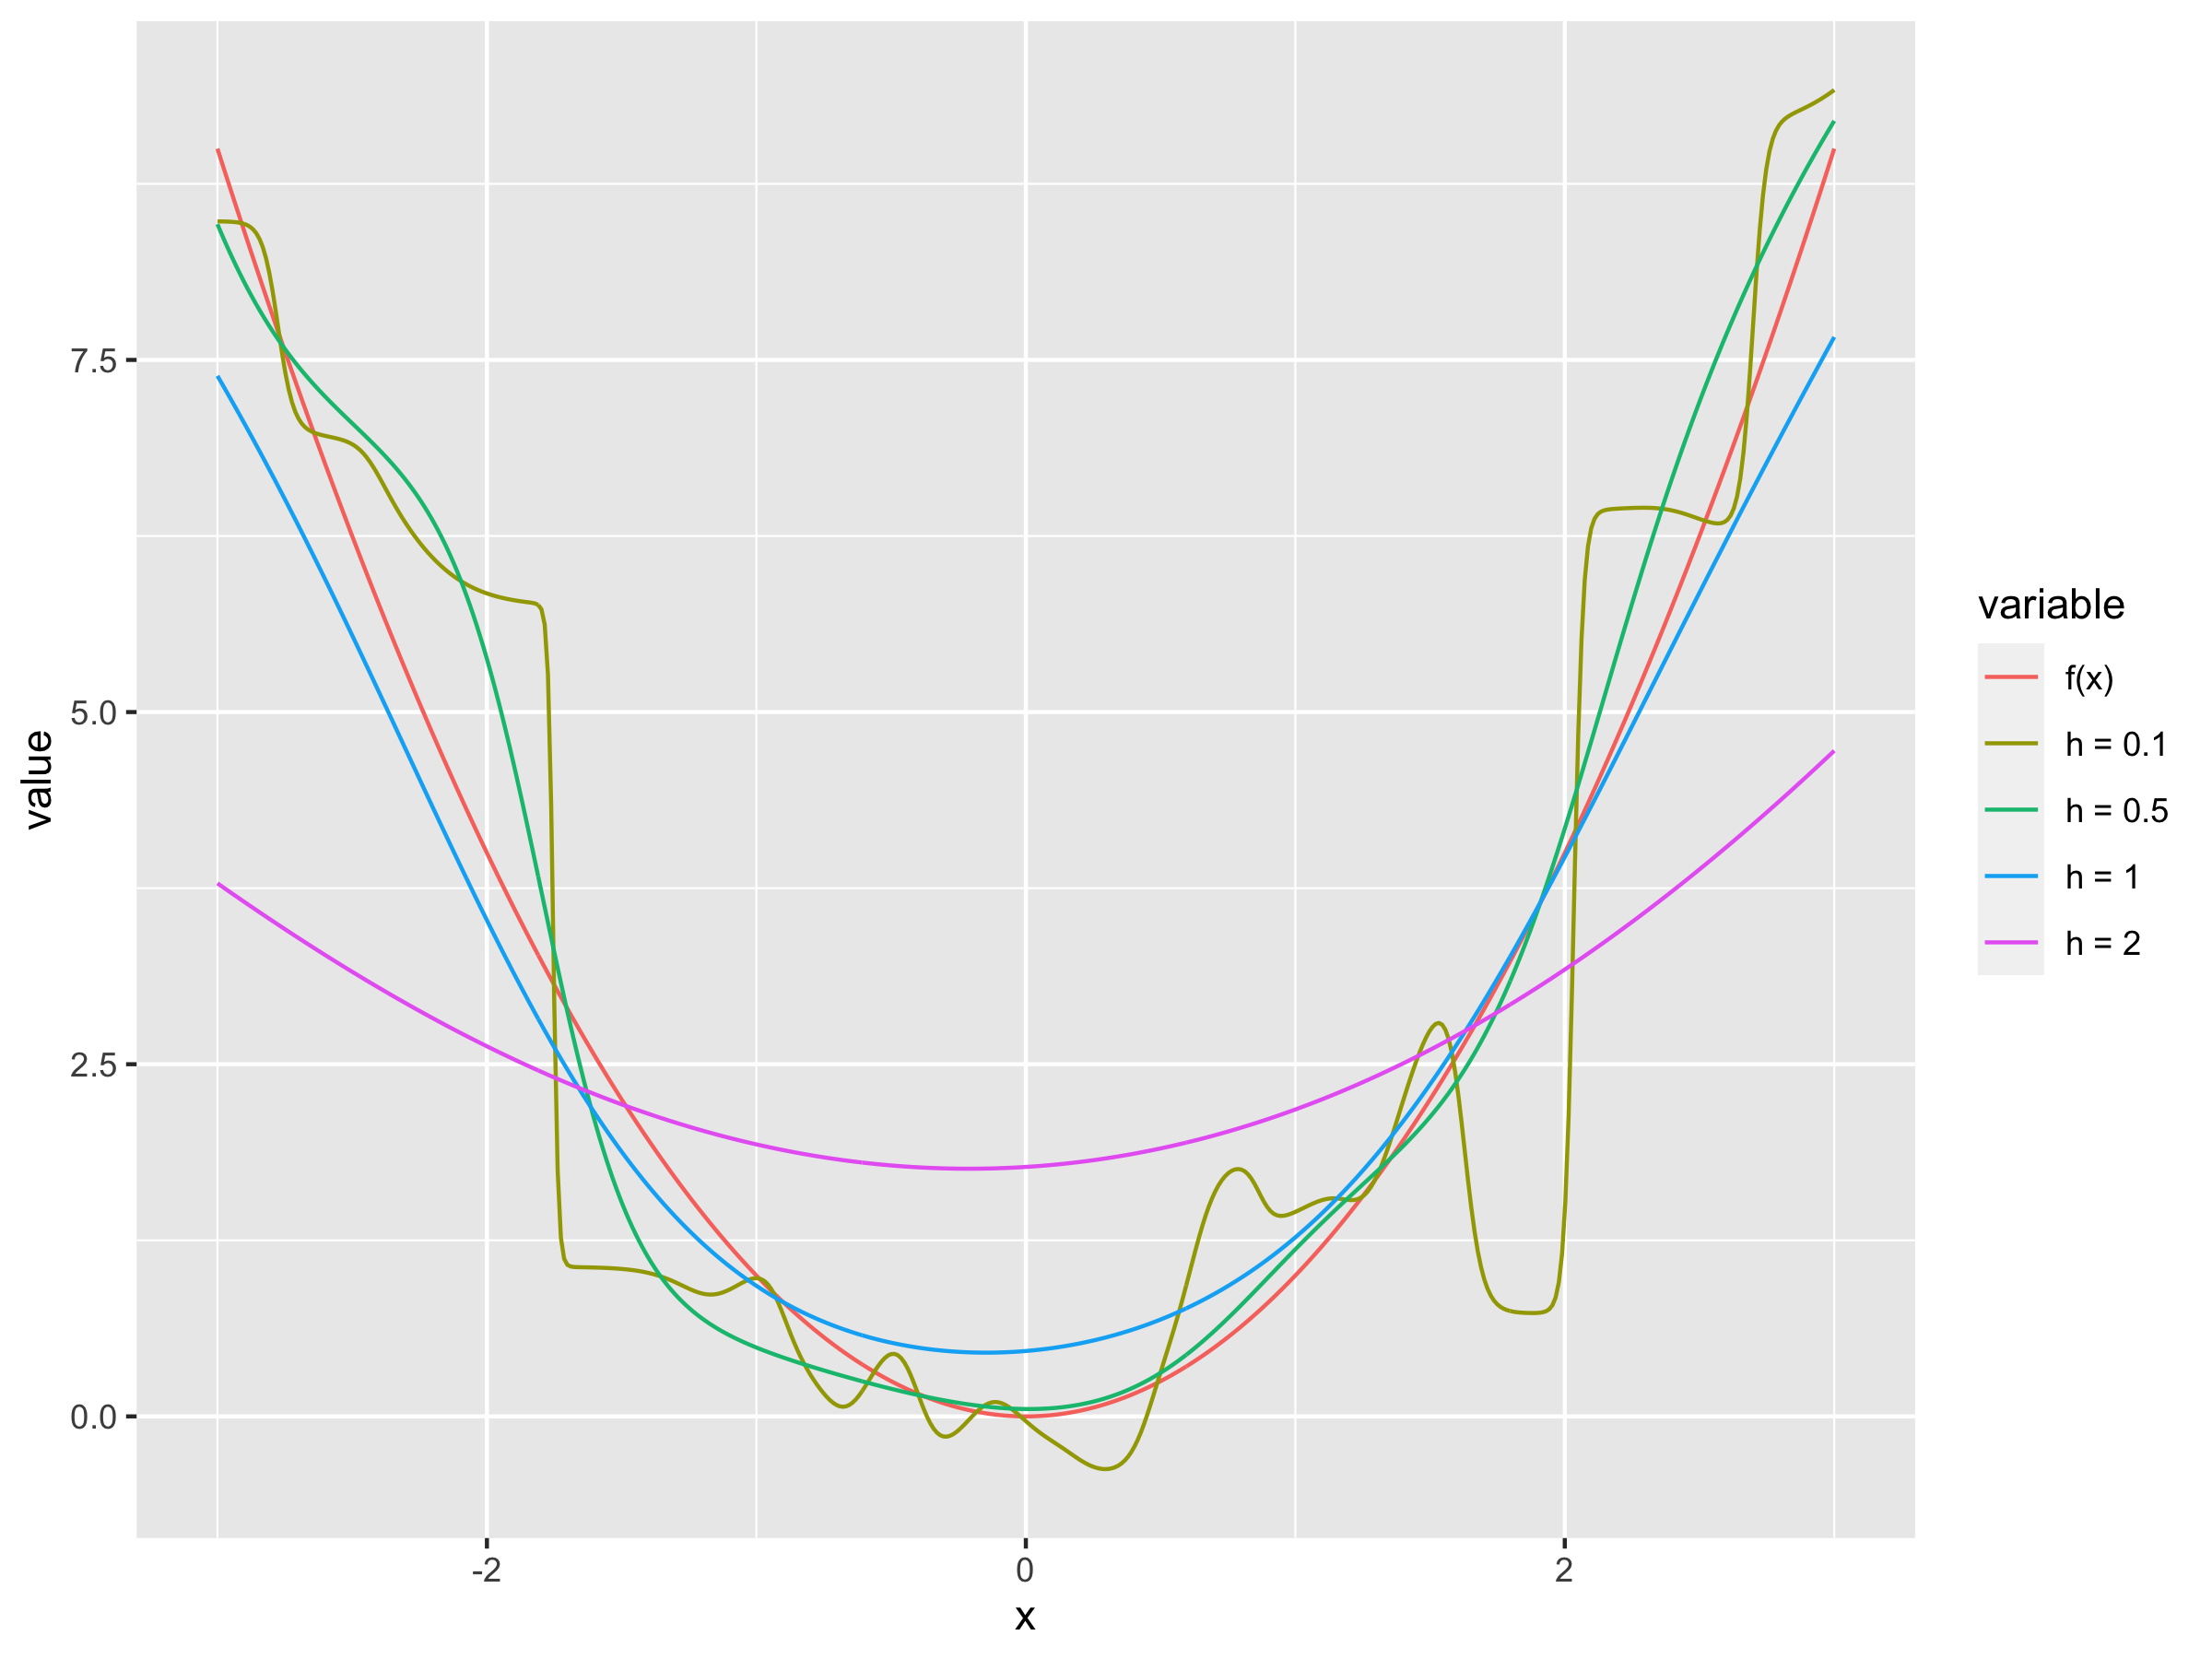
\includegraphics[width=0.8\textwidth]{Ex6/figures/kernel.png}
    \caption{Estimated Functions.}
    %\label{fig:hist_betai}
\end{figure}

\end{enumerate}

\newpage
\section{Cross validation}

Left unanswered so far in our previous study of kernel regression is the question: how does one choose the bandwidth $h$ used for the kernel?  Assume for now that the goal is to predict well, not necessarily to recover the truth.  (These are related but distinct goals.)  

\begin{enumerate}[(A)]


\item  Presumably a good choice of $h$ would be one that led to smaller predictive errors on fresh data.  Write a function or script that will: (1) accept an old (``training'') data set and a new (``testing'') data set as inputs; (2) fit the kernel-regression estimator to the training data for specified choices of $h$; and (3) return the estimated functions and the realized prediction error on the testing data for each value of $h$.  This should involve a fairly straightforward ``wrapper'' of the function you've already written.

\item Imagine a conceptual two-by-two table for the unknown, true state of affairs.  The rows of the table are ``wiggly function'' and ``smooth function,'' and the columns are ``highly noisy observations'' and ``not so noisy observations.''  Simulate one data set (say, 500 points) for each of the four cells of this table, where the $x$'s take values in the unit interval.  Then split each data set into training and testing subsets.  You choose the functions.\footnote{Trigonometric functions, for example, can be pretty wiggly if you make the period small.}   Apply your method to each case, using the testing data to select a bandwidth parameter.  Choose the estimate that minimizes the average squared error in prediction, which estimates the mean-squared error:
$$
L_n(\hat{f}) = \frac{1}{n}\sum_{i=1}^{n^{\star}} (y^{\star}_i - \hat{y}_i^{\star} )^2 \, ,
$$

where $(y_i^{\star}, x_i^{\star})$ are the points in the test set, and $ \hat{y}_i^{\star}$ is your predicted value arising from the model you fit using only the training data.  Does your out-of-sample predictive validation method lead to reasonable choices of $h$ for each case?

\bigskip \jie
We can tell from the results that, with high noise, we choose relatively large $h$ and for the lower noisy cases, the $h$ chosen are very small. The smooth and low noise case got fitted very well and the smooth, high noise, and wiggly, low noise cases are not bad. However, the wiggly with high noise case did not get the function estimated very well.

\begin{figure}[h]
    \centering
    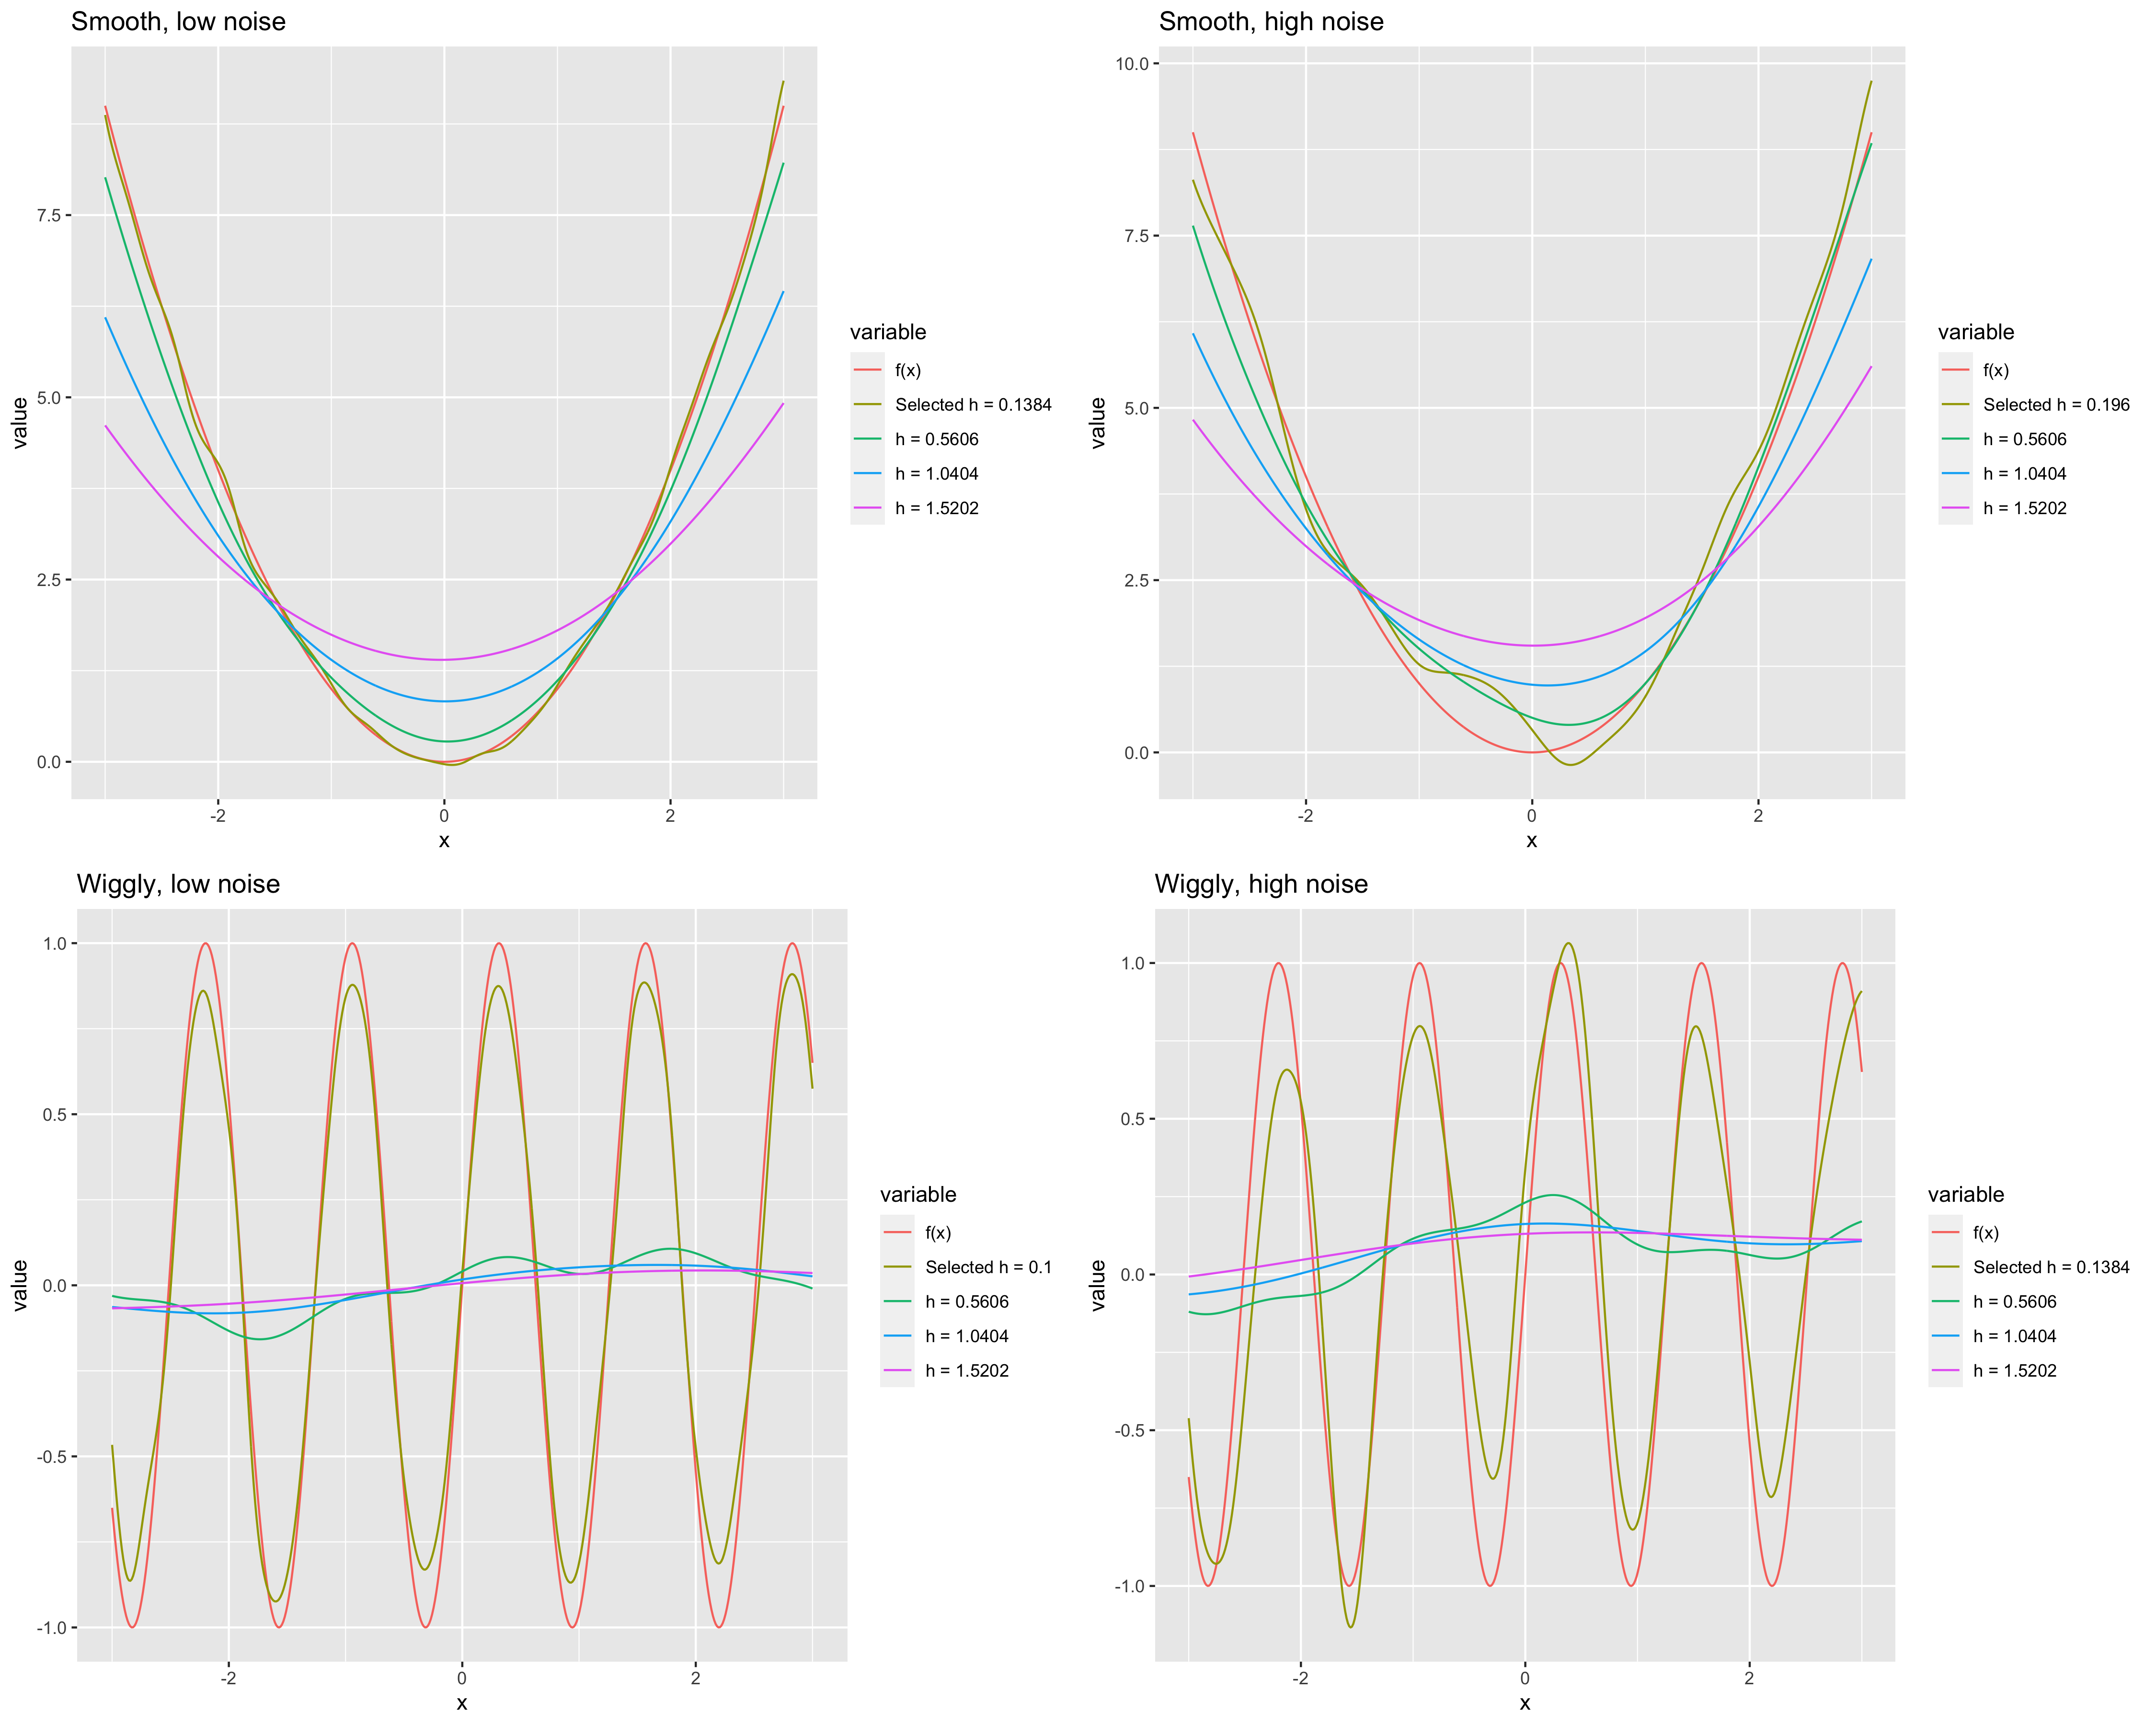
\includegraphics[width=\textwidth]{Ex6/figures/crossva.png}
    \caption{Estimated Functions.}
    %\label{fig:hist_betai}
\end{figure}

\item (optional problem,``leave-one-out lemma.'') Splitting a data set into two chunks to choose $h$ by out-of-sample validation has some drawbacks.  (See if you can think of two; one is obvious, one is more subtle.)  Then consider an alternative: leave-one-out cross validation.  Define
$$
\mbox{LOOCV} = \sum_{i=1}^n \left( y_i - \hat{y}_{i}^{(-i)} \right)^2 \, ,
$$
where $\hat{y}_{i}^{(-i)} $ is the predicted value of $y_i$ obtained by omitting the $i$th pair $(x_i, y_i)$ and fitting the model to the training data set of size $N-1$.\footnote{The intuition here is straightforward: for each possible choice of $h$, you have to predict each data point using all the others.  The bandwidth that with the lowest prediction error is the ``best'' choice by the LOOCV criterion.}  This $\hat{y}_{i}^{(-i)}$ is contingent upon a particular bandwidth, and is obviously a function of $x_i$, but these dependencies are suppressed for notational ease.  This error metric looks expensive to compute: for each value of $h$, and for each data point to be held out, it seems as though you must fit a whole nonlinear regression model.  But happily, there's a short-cut!

Observe that for a linear smoother, we can write the whole vector of fitted values as $\hat{y} = H y$, where $H$ is called the smoothing matrix (or ``hat matrix'') and $y$ is the vector of observed outcomes.\footnote{Remember that in linear regression fit by OLS, this is also true: $$\hat{y} = X \hat{\beta} = X (X^T X)^{-1} X^T y = Hy \, .$$}   Deduce that, for any linear smoother,
$$
\mbox{LOOCV} = \sum_{i=1}^n \left( \frac{  y_i - \hat{y}_{i} } {1-H_{ii}} \right)^2 \, .
$$

Hint: observe that for any matrix A whose rows\footnote{Remember that by default all vectors are column vectors. So when we write $a_i$, we mean the $i$th row of $A$ \emph{considered as a column vector}.  So as a row vector, it's $a_i^t$.} are $a_i^t, i = 1, \ldots n$, we have
$$
A^t A = \sum_{i=1}^n a_i a_i^t
$$
Therefore, if we let $X_{(-i)}$ be the original feature matrix with the $i$th row $x_i^t$ removed, we have
$$
X_{(-i)}^t X_{(-i)} = \sum_{l \neq i} x_i x_i^t = \sum_{l=1}^n x_l x_l^t  - x_i x_i^t = X'X - x_i x_i^t
$$
 This hint is useful because computing $\hat{y}_{i}^{(-i)}$ requires inverting $X_{(-i)}^t X_{(-i)}$.  This result, combined with the Sherman-Morrison formula, provides a path to do so, and ultimately to prove the leave-one-out lemma.  

Like I said, proving this lemma is optional. I will prove it in class, but consider it a nice linear algebra exercise to try to prove it yourself.  However, you should use it for the following part...

\item Use the leave-one-out lemma to revisit the examples you simulated in Part B, using leave-one-out cross validation to select $h$ in each case.  Because of the leave-one-out lemma, you won't need to actually refit the model N times!  

\begin{figure}[h]
    \centering
    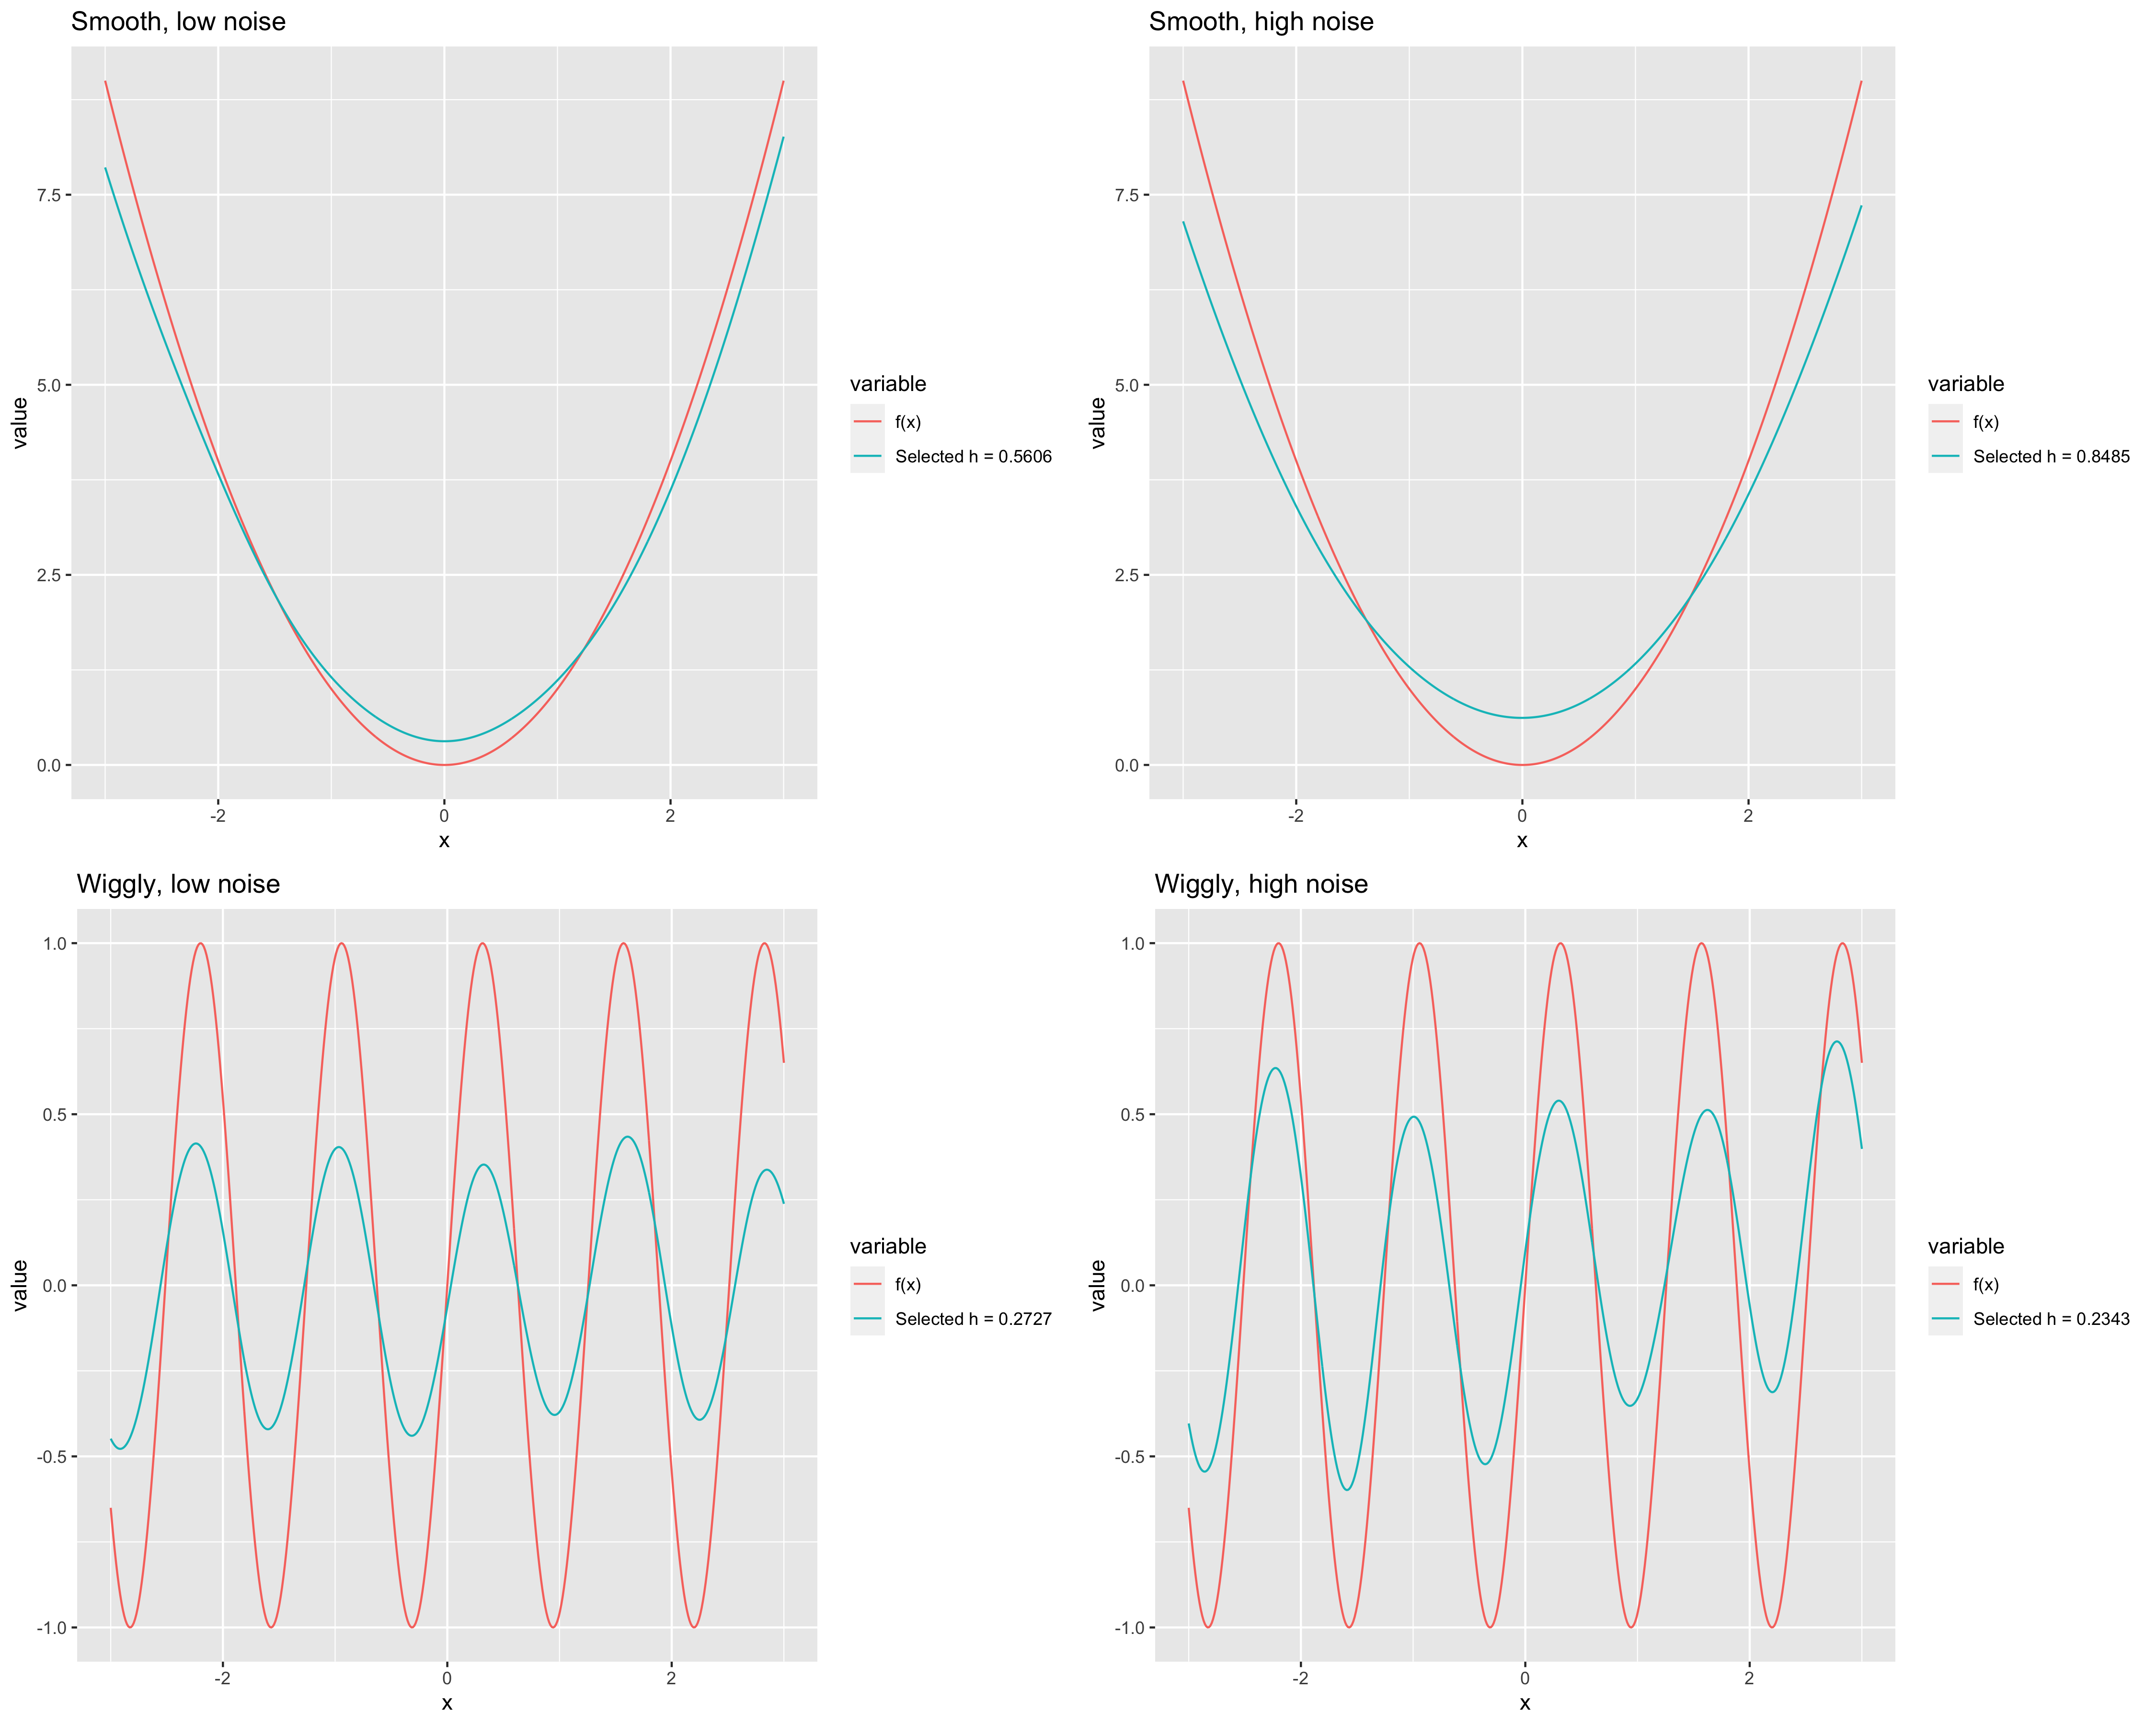
\includegraphics[width=\textwidth]{Ex6/figures/crossva_LOO.png}
    \caption{Estimated Functions.}
    %\label{fig:hist_betai}
\end{figure}

\end{enumerate}



\section{Local polynomial regression}

Kernel regression has a nice interpretation as a ``locally constant'' estimator, obtained from locally weighted least squares.  To see this, suppose we observe pairs $(x_i, y_i)$ for $i = 1, \ldots, n$ from our new favorite model, $y_i = f(x_i) + \epsilon_i$ and wish to estimate the value of the underlying function $f(x)$ at some point $x$ by weighted least squares.  Our estimate is the scalar\footnote{Because we are only talking about the value of the function at a specific point $x$, not the whole function.} quantity
$$
\hat{f}(x) = a = \arg \min_{\mathbb{R}} \sum_{i=1}^n w_i (y_i - a)^2 \, ,
$$
where the $w_i$ are the normalized weights (i.e.~they have been rescaled to sum to 1 for fixed $x$).  Clearly if $w_i = 1/n$, the estimate is simply $\bar{y}$, the sample mean, which is the ``best'' globally constant estimator.  Using elementary calculus, it is easy to see that if the unnormalized weights are
$$
w_i \equiv w(x, x_i) = \frac{1}{h} K \left( \frac{x_i - x}{h} \right)  \, ,
$$
then the solution is exactly the kernel-regression estimator.

\begin{enumerate}[(A)]

\item  A natural generalization of locally constant regression is local polynomial regression.  For points $u$ in a neighborhood of the target point $x$, define the polynomial
$$
g_{x}(u; a) = a_0 + \sum_{k=1}^D a_j(u-x)^k 
$$
for some vector of coefficients $a = (a_0, \ldots, a_D)$.  As above, we will estimate the coefficients $a$ in $g_{x}(u; a)$ at some target point $x$ using weighted least squares:
$$
\hat{a} = \arg \min_{R^{D+1}} \sum_{i=1}^n w_i \left\{ y_i - g_{x}(x_i; a)  \right\}^2 \, ,
$$
where $w_i \equiv w(x_i, x)$ are the kernel weights defined just above, normalized to sum to one.\footnote{We are fitting a different polynomial function for every possible choice of $x$.  Thus $\hat{a}$ depends on the target point $x$, but we have suppressed this dependence for notational ease.} Derive a concise (matrix) form of the weight vector $\hat{a}$, and by extension, the local function estimate $\hat{f}(x)$ at the target value $x$.\footnote{Observe that at the target point $x$, $g_x(u = x; a) = a_0$.  That is, only the constant term appears.  But this is not the same thing as fitting only a constant term!}   Life will be easier if you define the matrix $R_x$ whose $(i,j)$ entry is $(x_i-x)^{j-1}$, and remember that (weighted) polynomial regression is the same thing as (weighted) linear regression with a polynomial basis.

Note: if you get bogged down doing the general polynomial case, just try the linear case.

\item From this, conclude that for the special case of the local linear estimator ($D=1$), we can write $\hat{f}(x)$ as a linear smoother of the form
$$
\hat{f}(x) = \frac{\sum_{i=1}^n w_i(x) y_i }{\sum_{i=1}^n w_i(x)} \, ,
$$
where the unnormalized weights are
\begin{eqnarray*}
w_i(x) &=& K \left( \frac{x-x_i}{h} \right) \left\{  s_2(x) - (x_i-x) s_1(x) \right\}\\
s_j(x) &=& \sum_{i=1}^n K \left( \frac{x-x_i}{h} \right) (x_i-x)^j \, .
\end{eqnarray*}

\item Suppose that the residuals have constant variance $\sigma^2$ (that is, the spread of the residuals does not depend on $x$).  Derive the mean and variance of the sampling distribution for the local polynomial estimate $\hat{f}(x)$ at some arbitrary point $x$.  Note: the random variable $\hat{f}(x)$ is just a scalar quantity at $x$, not the whole function.

\item We don't know the residual variance, but we can estimate it.  A basic fact is that if $x$ is a random vector with mean $\mu$ and covariance matrix $\Sigma$, then for any symmetric matrix $Q$ of appropriate dimension, the quadratic form $x^T Q x$ has expectation
$$
E(x^T Q x) = \mbox{tr}(Q \Sigma) + \mu^T Q \mu \, .
$$
Write the vector of residuals as $r = y - \hat{y} = y - Hy$, where $H$ is the smoothing matrix.  Compute the expected value of the estimator
$$
\hat{\sigma}^2 = \frac{\Vert r \Vert_2^2}{n - 2\mbox{tr}(H) + \mbox{tr}(H^T H)} \, ,
$$
and simplify things as much as possible.  Roughly under what circumstances will this estimator be nearly unbiased for large $n$?  Note: the quantity $2\mbox{tr}(H) - \mbox{tr}(H^T H)$ is often referred to as the ``effective degrees of freedom'' in such problems.

\item Write code that fits the local linear estimator using a Gaussian kernel for a specified choice of bandwidth $h$. Then load the data in ``utilities.csv'' into R.\footnote{On the class GitHub site.}  This data set shows the monthly gas bill (in dollars) for a single-family home in Minnesota, along with the average temperature in that month (in degrees F), and the number of billing days in that month.  Let $y$ be the average daily gas bill in a given month (i.e.~dollars divided by billing days), and let $x$ be the average temperature.  Fit $y$ versus $x$ using local linear regression and some choice of kernel.  Choose a bandwidth by leave-one-out cross-validation.

\item Inspect the residuals from the model you just fit.  Does the assumption of constant variance (homoskedasticity) look reasonable?  If not, do you have any suggestion for fixing it?

\item Put everything together to construct an approximate point-wise 95\% confidence interval for the local linear model (using your chosen bandwidth) for the value of the function at each of the observed points $x_i$ for the utilities data.  Plot these confidence bands, along with the estimated function, on top of a scatter plot of the data.\footnote{It's fine to use Gaussian critical values for your confidence set.}

\end{enumerate}


\section{Gaussian processes}

A \textit{Gaussian process} is a collection of random variables $\{f(x): x \in \mathcal{X}\}$ such that, for any finite collection of indices $x_1, \ldots, x_N \in \mathcal{X}$, the random vector $[f(x_1), \ldots, f(x_N)]^T$ has a multivariate normal distribution.  It is a generalization of the multivariate normal distribution to infinite-dimensional spaces. The set $\mathcal{X}$ is called the index set or the state space of the process, and need not be countable.

A Gaussian process can be thought of as a random function defined over $\mathcal{X}$, often the real line or $\mathbb{R}^p$.  We write $f \sim \mbox{GP}(m, C)$ for some mean function $m: \mathcal{X} \rightarrow \mathbb{R}$ and a covariance function $C: \mathcal{X} \times \mathcal{X} \rightarrow \mathbb{R}^+$.  These functions define the moments\footnote{And therefore the entire distribution, because it is normal} of all finite-dimensional marginals of the process, in the sense that
$$
E\{ f(x_1) \} = m(x_1) \quad \mbox{and} \quad \mbox{cov}\{f(x_1), f(x_2) \} = C(x_1, x_2)
$$
for all $x_1, x_2 \in \mathcal{X}$.  More generally, the random vector $[f(x_1), \ldots, f(x_N)]^T$ has covariance matrix whose $(i,j)$ element is $C(x_i, x_j)$.  Typical covariance functions are those that decay as a function of increasing distance between points $x_1$ and $x_2$.  The notion is that $f(x_1)$ and $f(x_2)$ will have high covariance when $x_1$ and $x_2$ are close to each other.

\begin{enumerate}[(A)]
\item   Read up on the \href{https://en.wikipedia.org/wiki/Mat�rn_covariance_function}{Matern class}\footnote{\url{https://en.wikipedia.org/wiki/Matern_covariance_function}} of covariance functions.  The Matern class has the \textit{squared exponential} covariance function as a special case:
$$
C_{SE}(x_1, x_2) = \tau_1^2 \exp \left\{ - \frac{1}{2} \left( \frac{d(x_1, x_2)}{b} \right)^2 \right\} + \tau^2_2 \delta(x_1, x_2) \, ,
$$
where $d(x_1, x_2) = \Vert x_1 - x_2 \Vert_2$ is Euclidean distance (or just $|x-y|$ for scalars).  The constants $(b, \tau^2_1, \tau^2_2)$ are often called \textit{hyperparameters}, and $\delta(a,b)$ is the Kronecker delta function that takes the value 1 if $a=b$, and 0 otherwise.  But usually this covariance function generates functions that are ``too smooth,'' and so we use other covariance functions in the Matern class as a default.\footnote{See the speed comparison in kernel-benchmark.R on the class GitHub site if you want to see how Rcpp can be used to speed things up here.  My code is for the squared-exponential covariance function.}

Let's start with the simple case where $\mathcal{X} = [0,1]$, the unit interval.  Write a function that simulates a mean-zero Gaussian process on $[0,1]$ under the squared exponential covariance function.  The function will accept as arguments: (1) finite set of points $x_1, \ldots, x_N$ on the unit interval; and (2) a triplet $(b, \tau^2_1, \tau^2_2)$. It will return the value of the random process at each point: $f(x_1), \ldots, f(x_N)$.

Use your function to simulate (and plot) Gaussian processes across a range of values for $b$, $\tau^2_1$, and $\tau^2_2$.  Try starting with a very small value of $\tau^2_2$ (say, $10^{-6}$) and playing around with the other two first.  On the basis of your experiments, describe the role of these three hyperparameters in controlling the overall behavior of the random functions that result.  What happens when you try $\tau^2_2 = 0$? Why?  If you can fix this, do---remember our earlier discussion on different ways to simulate the MVN.

Now simulating a few functions with a different covariance function, the Mat\'ern with parameter $5/2$:
$$
C_{M52}(x_1, x_2) = \tau_1^2 \left\{ 1 + \frac{\sqrt{5}d}{b} + \frac{5d^2}{3b^2} \right\} \exp\left( \frac{-\sqrt{5}d}{b} \right) + \tau^2_2 \delta(x_1, x_2) \, ,
$$
where $d = \Vert x_1 - x_2 \Vert_2$ is the distance between the two points $x_1$ and $x_2$.  Comment on the differences between the functions generated from the two covariance kernels.

\item Suppose you observe the value of a Gaussian process $f \sim \mbox{GP}(m,C)$ at points $x_1, \ldots, x_N$.  What is the conditional distribution of the value of the process at some new point $x^{\star}$?  For the sake of notational ease simply write the value of the $(i,j)$ element of the covariance matrix as $C_{i,j}$, rather than expanding it in terms of a specific covariance function.

\item Prove the following lemma.

\begin{lemma}
Suppose that the joint distribution of two vectors $y$ and $\theta$ has the following properties: (1) the conditional distribution for $y$ given $\theta$ is multivariate normal, $(y \mid \theta) \sim N(R\theta, \Sigma)$; and (2) the marginal distribution of $\theta$ is multivariate normal, $\theta \sim N(m,V)$.  Assume that $R$, $\Sigma$, $m$, and $V$ are all constants.  Then the joint distribution of $y$ and $\theta$ is multivariate normal.
\end{lemma}

\end{enumerate}


\section{In nonparametric regression and spatial smoothing}

\begin{enumerate}[(A)]

\item Suppose we observe data $y_i = f(x_i) + \epsilon_i$, $\epsilon_i \sim N(0, \sigma^2)$, for some unknown function $f$. Suppose that the prior distribution for the unknown function is a mean-zero Gaussian process: $f \sim \mbox{GP}(0, C)$ for some covariance function $C$.  Let $x_1, \ldots, x_N$ denote the previously observed $x$ points.  Derive the posterior distribution for the random vector $[f(x_1), \ldots, f(x_N)]^T$, given the corresponding outcomes $y_1, \ldots, y_N$, assuming that you know $\sigma^2$.

\item As before, suppose we observe data $y_i = f(x_i) + \epsilon_i$, $\epsilon_i \sim N(0, \sigma^2)$, for $i=1, \ldots, N$.  Now we wish to predict the value of the function $f(x^{\star})$ at some new point $x^{\star}$ where we haven't seen previous data.  Suppose that $f$ has a mean-zero Gaussian process prior, $f \sim GP(0, C)$.  Show that the posterior mean $E\{ f(x^{\star}) \mid y_1, \ldots, y_N \}$ is a linear smoother, and derive expressions both for the smoothing weights and the posterior variance of $f(x^{\star})$.

\item Go back to the utilities data, and plot the pointwise posterior mean and 95\% posterior confidence interval for the value of the function at each of the observed points $x_i$ (again, superimposed on top of the scatter plot of the data itself).  Choose $\tau^2_2$ to be very small, say $10^{-6}$, and choose $(b, \tau^2_1)$ that give a sensible-looking answer.\footnote{If you're bored with the utilities data, instead try the data in ethanol.csv, in which the NOx emissions of an ethanol engine are measured as the engine's fuel-air equivalence ratio (E in the data set) is varied.  Your goal would be to model NOx as a function of E using a Gaussian process. }

\item Let $y_i = f(x_i) + \epsilon_i$, and suppose that $f$ has a Gaussian-process prior under the Matern(5/2) covariance function $C$ with scale $\tau^1_2$, range $b$, and nugget $\tau^2_2$.  Derive an expression for the marginal distribution of $y = (y_1 \ldots, y_N)$ in terms of $(\tau^2_1, b, \tau^2_2)$, integrating out the random function $f$.  This is called a marginal likelihood.

\item Return to the utilities or ethanol data sets. Fix $\tau^2_2 = 0$, and evaluate the log of the marginal likelihood function $p(y \mid \tau^2_1, b)$ over a discrete 2-d grid of points.\footnote{Don't just use a black-box optimizer; we want to make sure we get the best solution if there are multiple modes.} If you're getting errors in your code with $\tau^2_2 = 0$, use something very small instead.  Use this plot to choose a set of values $(\hat{\tau^2_1}, \hat{b})$ for the hyperparameters.  Then use these hyperparameters to compute the posterior mean for $f$, given $y$.  Comment on any lingering concerns you have with your fitted model.

\item In \verb|weather.csv| you will find data on two variables from 147 weather stations in the American Pacific northwest.
\begin{compactdesc}
\item[pressure]: the difference between the forecasted pressure and the actual pressure reading at that station (in Pascals)
\item[temperature]: the difference between the forecasted temperature and the actual temperature reading at that station (in Celsius)
\end{compactdesc}
There are also latitude and longitude coordinates of each  station.  Fit a Gaussian process model for each of the temperature and pressure variables.  Choose hyperparameters appropriately.  Visualize your fitted functions (both the posterior mean and posterior standard deviation) on a regular grid using something like a contour plot or color image.  Read up on the \verb|image|, \verb|filled.contour|, or \verb|contourplot|\footnote{in the lattice library} functions in R.  An important consideration: is Euclidean distance the appropriate measure to go into the covariance function?  Or do we need separate length scales for the two dimensions, i.e.
$$
d^2(x, z) = \frac{(x_1 - z_1)^2}{b_1^2} +  \frac{(x_2 - z_2)^2}{b_2^2} \, .
$$
Justify your reasoning for using Euclidean distance or this ``nonisotropic'' distance.


%\item In \verb|droslong.csv|, you will find a small subset of a time-course DNA microarray experiment.  The gene-expression profiles of 2000 different genes in the fruit fly (Drosophila) genome are tracked over time during embryogenesis; you are getting data on 14 of these genes, organized in three groups (think of these as marking which cellular pathway that gene influences).  For each gene at each time point, there are 3 ``technical replicates''---that is, three copies of the same biological material from the same fly, run through the same process to measure gene expression.
%
%The question of interest is: how does each gene's expression profile change over time, as the process of embryogenesis unfolds?  Propose a hierarchical model for this data that properly reflects its structure.
%
%A nice graphics package is the ``lattice'' library.  Install and load this; then try commands such as
%\begin{verbatim}
%xyplot(log2exp~time | gene, data=droslong)
%xyplot(log2exp~time | group, data=droslong)
%\end{verbatim}
%to begin exploring the structure of this data.

\end{enumerate}



\end{document}
